\documentclass[10pt, compress, aspectratio=169]{beamer}

\usetheme[numbering=fraction, progressbar=none, titleformat=smallcaps, sectionpage=none]{metropolis}

\usepackage{sourcecodepro}
\usepackage{booktabs}
\usepackage{array}
\usepackage{listings}
\usepackage{graphicx}
\usepackage{import}
\usepackage[english]{babel}
\usepackage[scale=2]{ccicons}
\usepackage{url}
\usepackage{relsize}
\usepackage{wasysym}

\usepackage{pgfplots}
\usepgfplotslibrary{dateplot}

\definecolor{Base}{HTML}{191F26}
\definecolor{Accent}{HTML}{157FFF}

\setbeamercolor{alerted text}{fg=Accent}
\setbeamercolor{frametitle}{bg=Base}

\setsansfont[BoldFont={Source Sans Pro Semibold},
              Numbers={OldStyle}]{Source Sans Pro}

\lstset{ %
  backgroundcolor={},
  basicstyle=\ttfamily\footnotesize,
  breakatwhitespace=true,
  breaklines=true,
  captionpos=n,
  commentstyle=\color{orange},
  escapeinside={\%*}{*)},
  extendedchars=true,
  frame=n,
  keywordstyle=\color{Accent},
  language=C++,
  rulecolor=\color{black},
  showspaces=false,
  showstringspaces=false,
  showtabs=false,
  stepnumber=2,
  stringstyle=\color{gray},
  tabsize=2,
  keywords={thrust,plus,device_vector, copy,transform,begin,end, copyin,
  copyout, acc, \_\_global\_\_, void, int, float, main, threadIdx, blockIdx,
  blockDim, if, else, malloc, NULL, cudaMalloc, cudaMemcpy, cudaSuccess,
  cudaGetLastError, cudaDeviceSynchronize, cudaFree, cudaMemcpyDeviceToHost,
  cudaMemcpyHostToDevice, const, data, independent, kernels, loop,
  fprintf, stderr, cudaGetErrorString, EXIT_FAILURE, for, dim3},
  otherkeywords={::, \#pragma, \#include, <<<,>>>, \&, \*, +, -, /, [, ], >, <}
}

\renewcommand*{\UrlFont}{\ttfamily\smaller\relax}

\graphicspath{{../img/}}

\title{Autotuning for High Performance Computing}
\author{\footnotesize Pedro Bruel \\ {\scriptsize \emph{phrb@ime.usp.br}}}
\institute{
\includegraphics[height=2cm]{imelogo}\\[0.2cm] Instituto de Matemática e Estatística \\ Universidade de São Paulo}
\date{\scriptsize \today}

\begin{document}

\maketitle

\section*{Introduction}

\subsection*{About}

\begin{frame}
    \frametitle{About}
    \begin{columns}[T,onlytextwidth]
        \column{0.5\textwidth}
        \begin{center}
            \includegraphics[width=.32\textwidth]{pedro}

            Pedro Bruel

            \textit{phrb@ime.usp.br}
        \end{center}

        \begin{center}
            \includegraphics[width=.34\textwidth]{sai}

            Sai Rahul Chalamalasetti

            \textit{sairahul.chalamalasetti@hpe.com}
        \end{center}

        \column{0.5\textwidth}
        \begin{center}
            \includegraphics[width=.3\textwidth]{alfredo}

            Alfredo Goldman

            \textit{gold@ime.usp.br}
        \end{center}

        \begin{center}
            \includegraphics[width=.32\textwidth]{dejan}

            Dejan Milojicic

            \textit{dejan.milojicic@hpe.com}
        \end{center}

    \end{columns}
\end{frame}

\subsection*{Outline}

\begin{frame}
    \frametitle{Outline}
    \setbeamertemplate{section in toc}[sections numbered]
    \tableofcontents[hideallsubsections]
\end{frame}

\begin{frame}
    \frametitle{Slides}
    \begin{center}
        \includegraphics[width=.18\textwidth]{github}
    \end{center}
    Slides are hosted at \alert{GitHub}:

    \begin{itemize}
        \item \url{github.com/phrb/autotuning-for-hpc}
    \end{itemize}
\end{frame}

\section{Autotuning}

\begin{frame}
    \frametitle{Autotuning: Optimization as a Search Problem}
    Casting \alert{program optimization} as a \alert{search problem}:

    \alert{Search Spaces}:
    \begin{itemize}
        \item Algorithm Selections
        \item Program Configurations
        \item $\dots$
    \end{itemize}

    \alert{Search Objectives}:
    \begin{itemize}
        \item Minimize \alert{execution time}
        \item Maximize \alert{usage of resources}
        \item $\dots$
    \end{itemize}
\end{frame}

\begin{frame}
    \frametitle{Autotuning: Optimization as a Search Problem}
    \begin{table}[]
        \centering
        \begin{tabular}{@{}lll@{}}
            \toprule
            Domain & Search Space & Search Objective \\ \midrule
            LLVM Compiler & Ordering and Parameters of Optimizations & Size, time, memory, $\dots$ \\
            Genetic Algorithms & Configuration Parameters & Time to find solution \\
            Sorting & Size to switch to Insertion Sort & Execution time \\
            Machine Learning & Model selection and parameters & Model accuracy \\
            DSP Algorithms & Algorithm Parameters & Accuracy, execution time, $\dots$ \\ \bottomrule
        \end{tabular}
        \caption{Sample of autotuning domains, possible search spaces and objectives}
    \end{table}
\end{frame}

\begin{frame}
    \frametitle{Search Spaces \& Techniques}
    The \alert{search spaces} created by program optimization problems can be
    \alert{difficult to explore}

    \begin{center}
        \includegraphics[width=.6\textwidth]{rastrigin}

        Rastrigin function, with \alert{global minimum} $f(0,0) = 0$
    \end{center}
\end{frame}

\begin{frame}
    \frametitle{Search Spaces \& Techniques}
    \begin{table}[]
        \centering
        \begin{tabular}{@{}lll@{}}
            \toprule
            System & Domain & Search Technique \\ \midrule
            ATLAS & Dense Linear Algebra & Exhaustive \\
            Insieme & Compiler & Genetic Algorithm \\
            SPIRAL & DSP Algorithms & Pareto Active Learning \\
            Active Harmony & Runtime & Nelder-Mead \\ \bottomrule
        \end{tabular}
        \caption{Sample of autotuning systems, their domains and techniques}
    \end{table}

    \begin{itemize}
        \item Different \alert{problem domains} generate different \alert{search spaces}
        \item \alert{No single solution} for all domains
        \item Search techniques can be composed: \alert{OpenTuner}
        \item Independent searches can be \alert{parallelized and distributed}
    \end{itemize}
\end{frame}

\begin{frame}
    \frametitle{Autotuning: Abstract Model}
    \begin{center}
        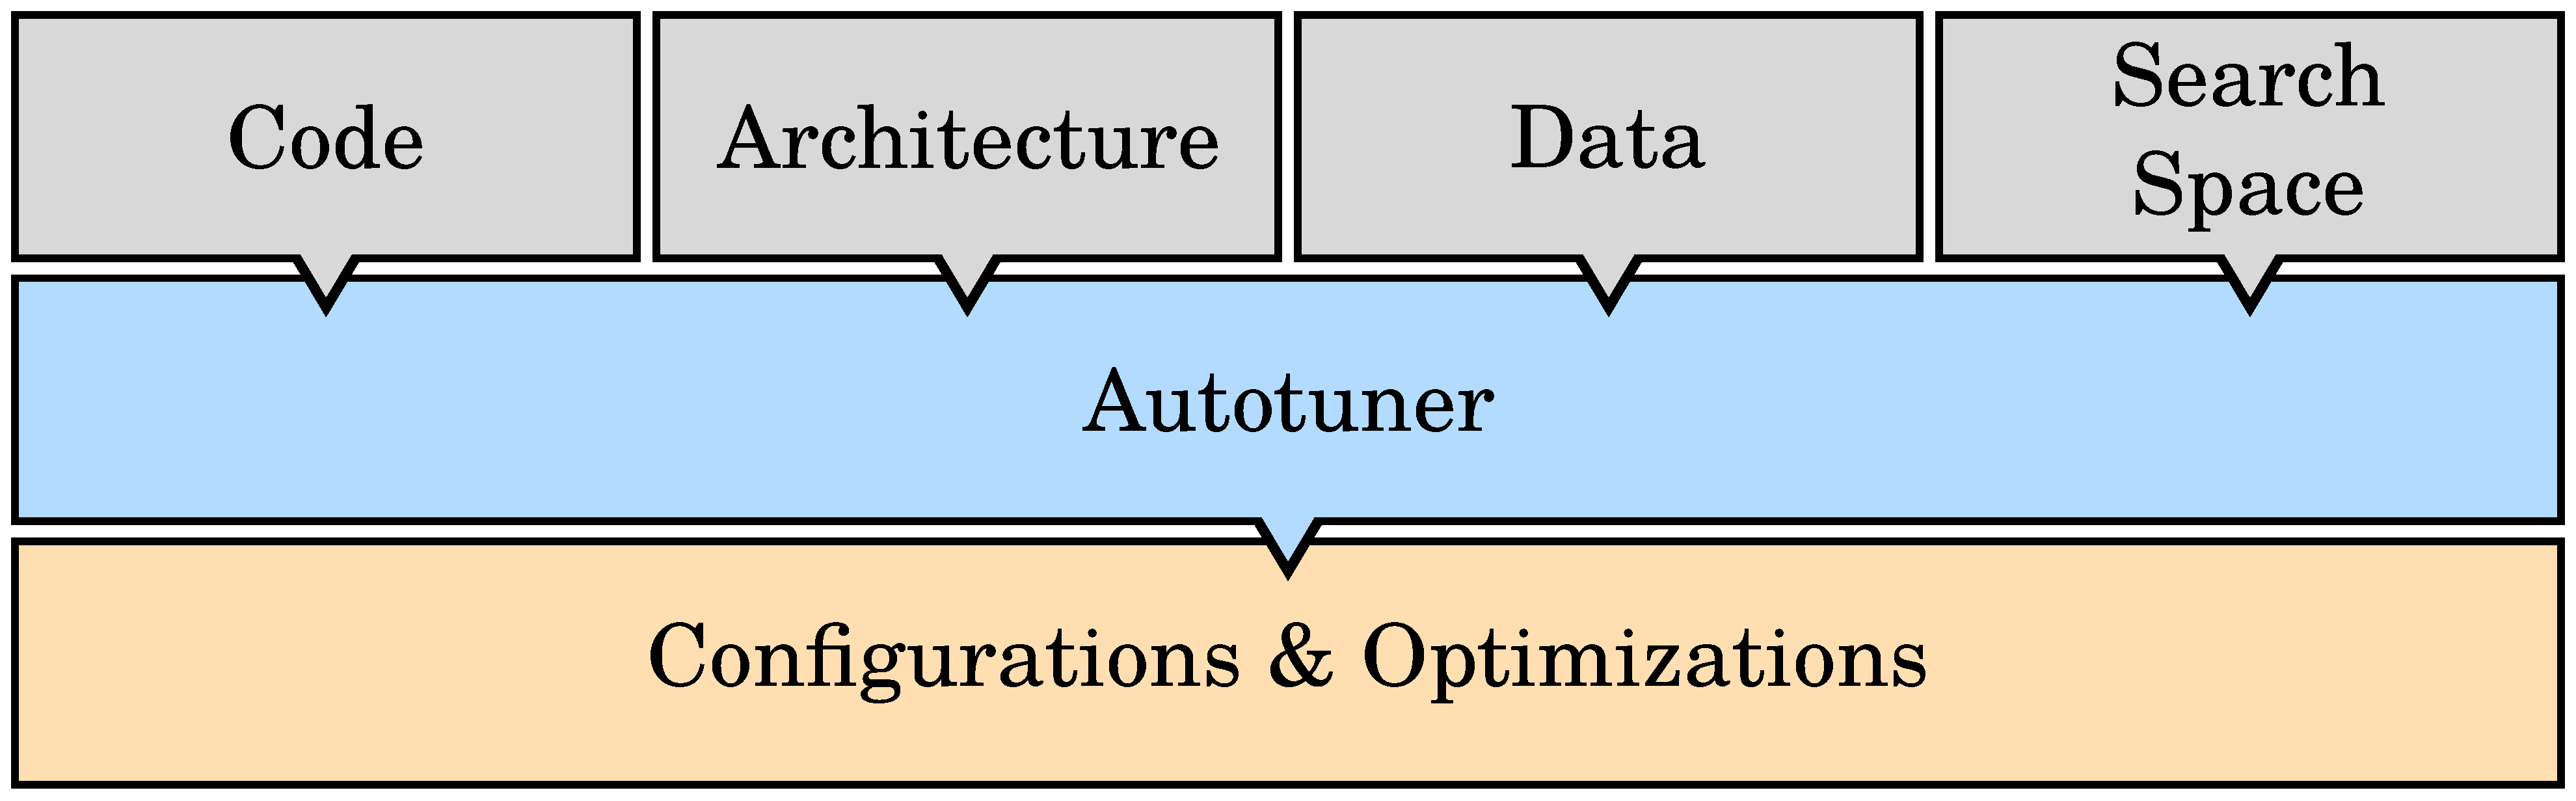
\includegraphics[width=.5\textwidth]{overview}
    \end{center}
\end{frame}

\section{Autotuning GPU Compiler Parameters}

\begin{frame}
    \frametitle{NVIDIA CUDA Compiler: From CUDA C++ to Object Code}
    \begin{center}
        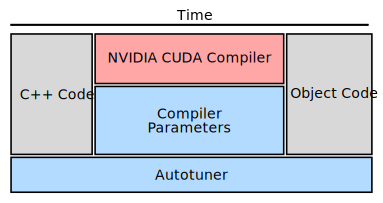
\includegraphics[width=.6\textwidth]{gpu-stack}
    \end{center}

    \begin{itemize}
        \item We tuned applications from the \alert{Rodinia Benchmark Suite}
        \item C++ $\rightarrow$ Object Code: takes \alert{seconds}; \alert{up to 4x speedup}
        \item We \alert{tuned the parameters} of the NVIDIA CUDA Compiler (NVCC)
    \end{itemize}
\end{frame}

\begin{frame}
    \frametitle{Autotuning: GPUs}
    \begin{center}
        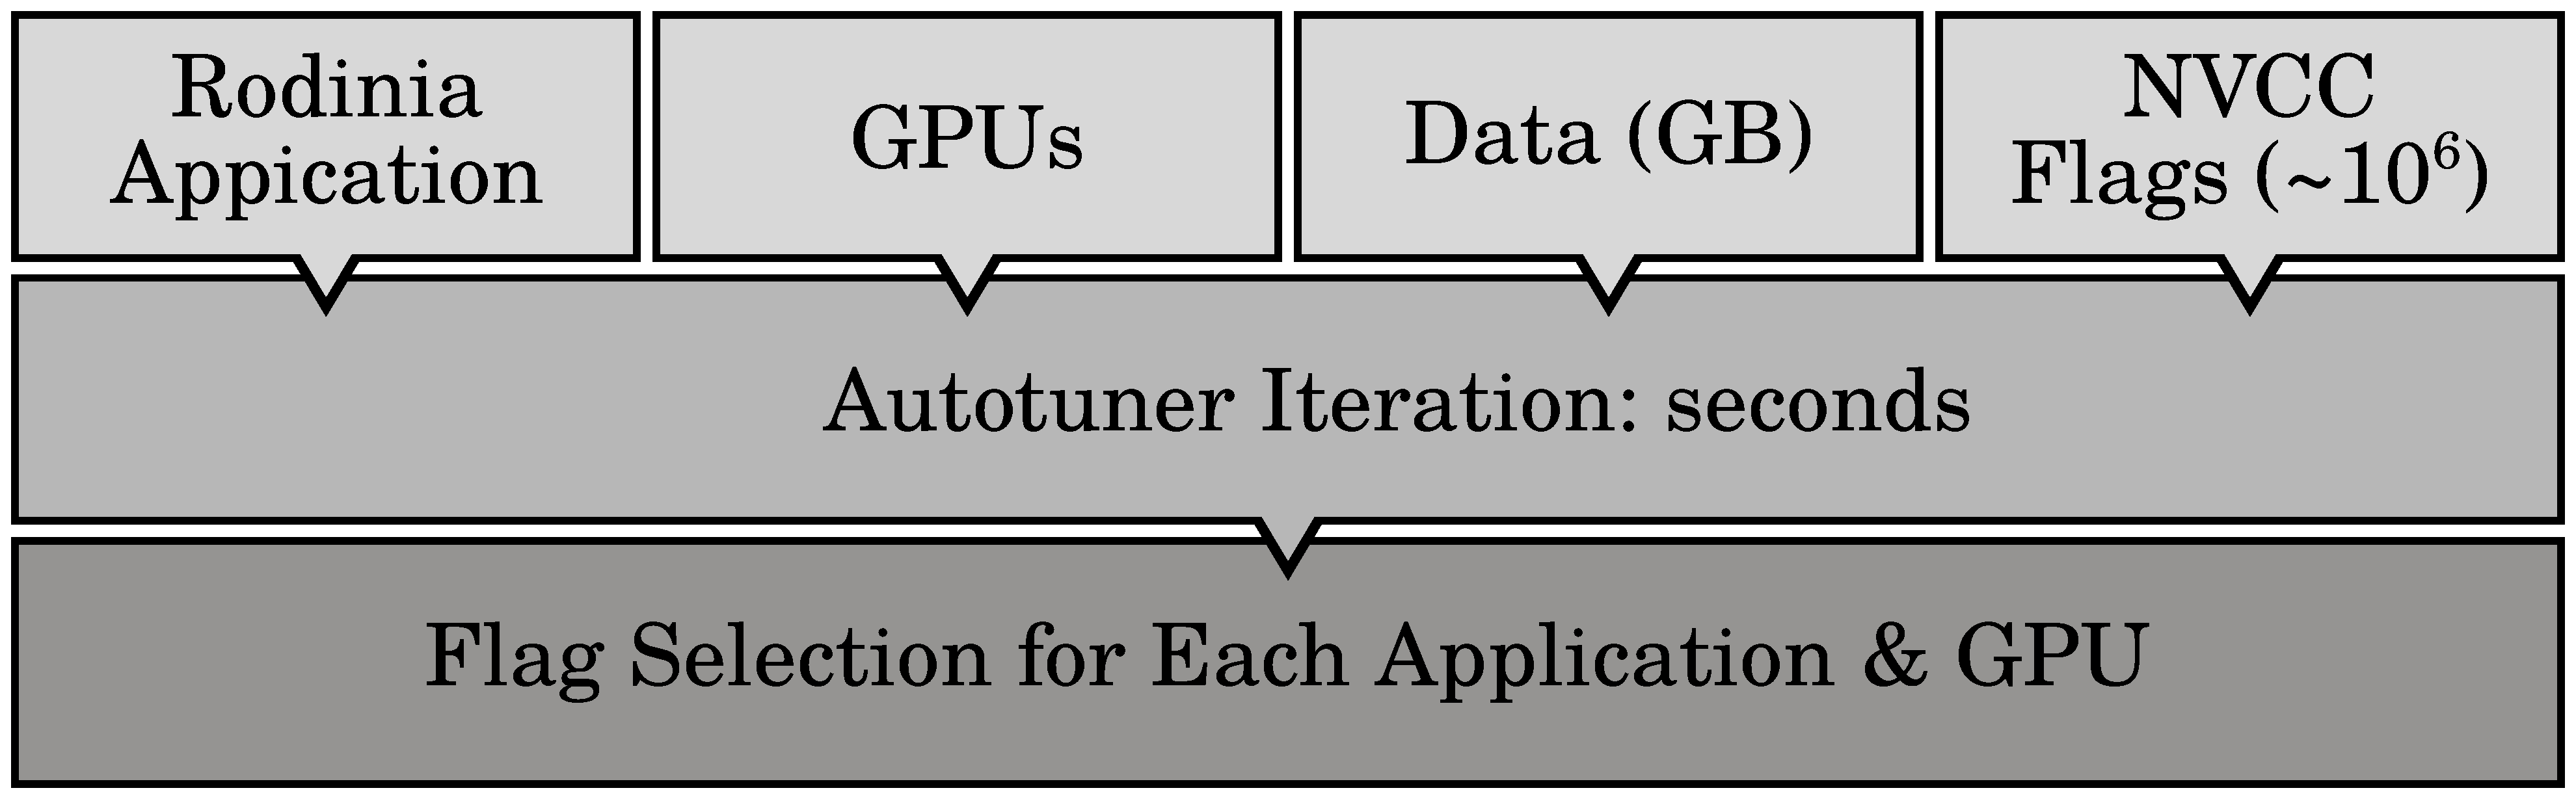
\includegraphics[width=.73\textwidth]{overview_gpus}

        \alert{1h} of tuning $\rightarrow \; \dfrac{3600s}{\sim{}s} \approx \alert{10^3}$ \alert{iterations}
    \end{center}
\end{frame}

\begin{frame}
    \frametitle{Results}
    \alert{Most significative speedups} for \alert{Rodinia applications}, on the left,
    and \alert{matrix multiplication optimizations}, on the right, after \alert{1.5h of tuning}:
    \begin{columns}[T,onlytextwidth]
        \column{0.5\textwidth}
        \vspace{0.57cm}
        \begin{center}
            \includegraphics[width=.9\textwidth]{RodiniaSummary}
        \end{center}

        \column{0.5\textwidth}
        \begin{center}
            \includegraphics[width=.9\textwidth]{MatrixSummary}
        \end{center}

    \end{columns}
    We \alert{found no globally good parameter selections} for specific GPUs or applications
\end{frame}

\section{Autotuning High-Level Synthesis for FPGAs}

\begin{frame}
    \frametitle{High-Level Synthesis for FPGAs: From C to Hardware}
    \begin{center}
        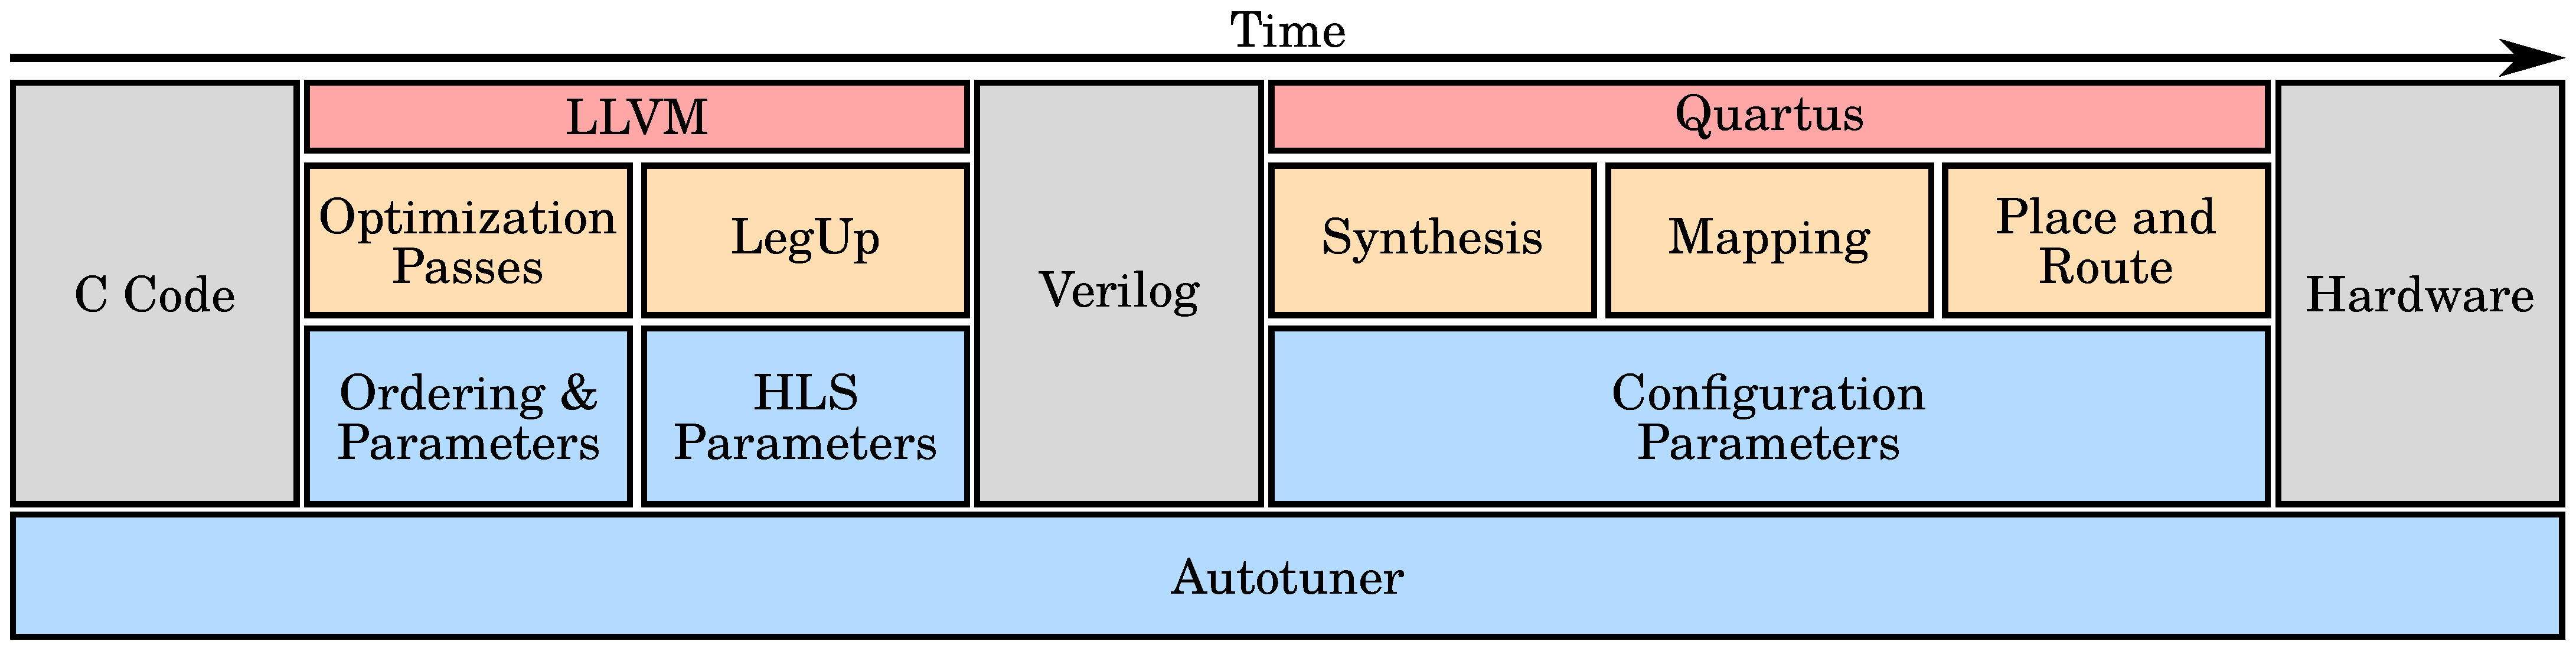
\includegraphics[width=1\textwidth]{fpga-stack-all-colors}
    \end{center}

    \begin{itemize}
        \item We tuned applications from the \alert{CHStone Benchmark Suite}
        \item C $\rightarrow$ Verilog: takes \alert{seconds}; \alert{\textasciitilde16\% speedup}
        \item Verilog $\rightarrow$ Hardware: takes \alert{minutes}, \alert{hours}; \alert{10\%-2x speedup}
        \item We tuned C $\rightarrow$ Verilog, but had \alert{to pay the cost} of Verilog $\rightarrow$ Hardware
    \end{itemize}
\end{frame}

\begin{frame}
    \frametitle{High-Level Synthesis for FPGAs: From C to Hardware}
    \begin{center}
        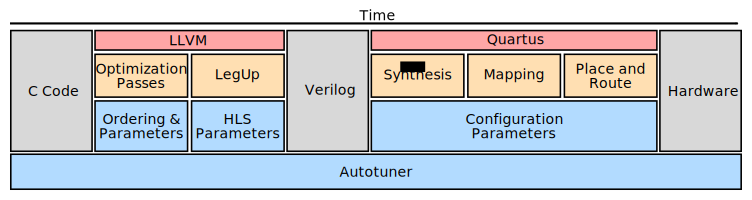
\includegraphics[width=1\textwidth]{fpga-stack}
    \end{center}

    \begin{itemize}
        \item We tuned applications from the \alert{CHStone Benchmark Suite}
        \item C $\rightarrow$ Verilog: takes \alert{seconds}; \alert{\textasciitilde16\% speedup}
        \item Verilog $\rightarrow$ Hardware: takes \alert{minutes}, \alert{hours}; \alert{10\%-2x speedup}
        \item We tuned C $\rightarrow$ Verilog, but had \alert{to pay the cost} of Verilog $\rightarrow$ Hardware
    \end{itemize}
\end{frame}

\begin{frame}
    \frametitle{Autotuning LegUp Parameters for CHStone}
    \begin{center}
        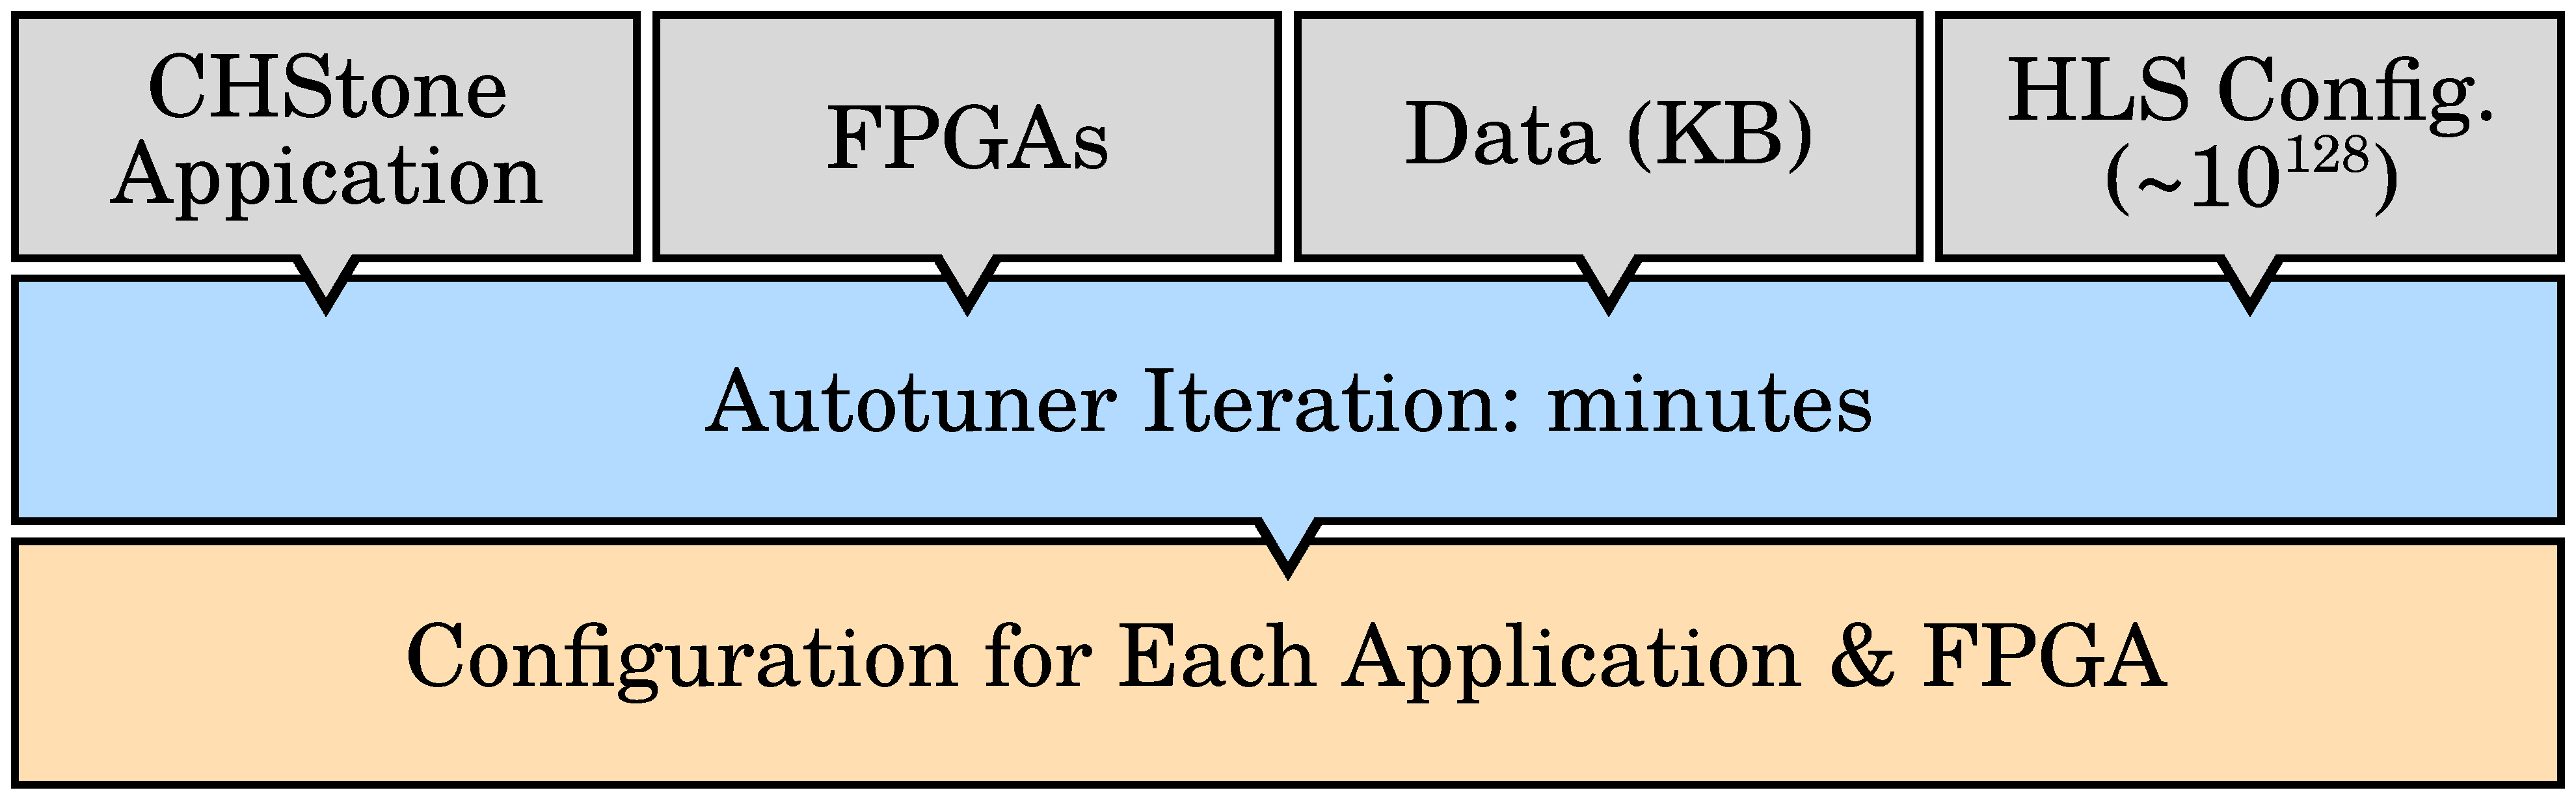
\includegraphics[width=.73\textwidth]{overview_fpgas_small}

         \alert{1h} of tuning $\rightarrow \; \dfrac{60min}{\sim{}min} \approx \alert{10}$ \alert{iterations}
    \end{center}
\end{frame}

\begin{frame}
    \frametitle{Autotuning LegUp Parameters for CHStone}
    \alert{Search Space}:
    \begin{itemize}
        \item \alert{LegUp constraints} that impact \alert{Verilog generation}
        \item Read from a \alert{configuration file}
    \end{itemize}

    Examples:
    \begin{itemize}
        \item \texttt{set\_accelerator\_function}
        \item \texttt{ENABLE\_PATTERN\_SHARING}
    \end{itemize}

    \begin{center}
        \tiny{Source: \url{legup.eecg.utoronto.ca/docs/4.0/constraintsmanual.html\#constraints} [Accessed on 15/09/16]}
    \end{center}
\end{frame}

\begin{frame}
    \frametitle{Autotuning LegUp Parameters for CHStone}
    Calculating the \alert{fitness function}:

    \begin{itemize}
        \item $M$: the set of \alert{metrics}
        \item $W$: the set of \alert{weights for each metric}
        \item $m_{i}^{0}$: \alert{initial measured value} for each metric
        \item $f(M,W)$: \alert{cost} or \alert{fitness function}, defined as
    \end{itemize}
    \begin{align*}
        f(M, W) = \dfrac{\sum\limits_{\substack{m_i \in M \\ w_i \in W}}{w_i\Big(\dfrac{m_i}{m_{i}^{0}}\Big)}}{\sum\limits_{w_i \in W}{w_i}}
    \end{align*}
    \begin{itemize}
        \item \alert{Naive weights}: $w_i = 1, \; \forall w_i \in W$
    \end{itemize}
\end{frame}

\begin{frame}
    \frametitle{Results}
    Relative variation for the \alert{individual metrics} of the \alert{dfdiv}
    CHStone application, during \alert{1.5h of tuning}:
    \begin{columns}[T,onlytextwidth]
        \column{0.5\textwidth}
        \begin{center}
            \includegraphics[width=.92\textwidth]{dfmul_all_5400_chstone_StratixV}
        \end{center}

        \column{0.5\textwidth}
        \begin{center}
            \includegraphics[width=.92\textwidth]{dfmul_all_5400_chstone_CycloneV}
        \end{center}

    \end{columns}
\end{frame}

\begin{frame}
    \frametitle{Results}
    Relative variation for the \alert{individual metrics} of the \alert{adpcm}
    CHStone application, during \alert{1.5h of tuning}:
    \begin{columns}[T,onlytextwidth]
        \column{0.5\textwidth}
        \begin{center}
            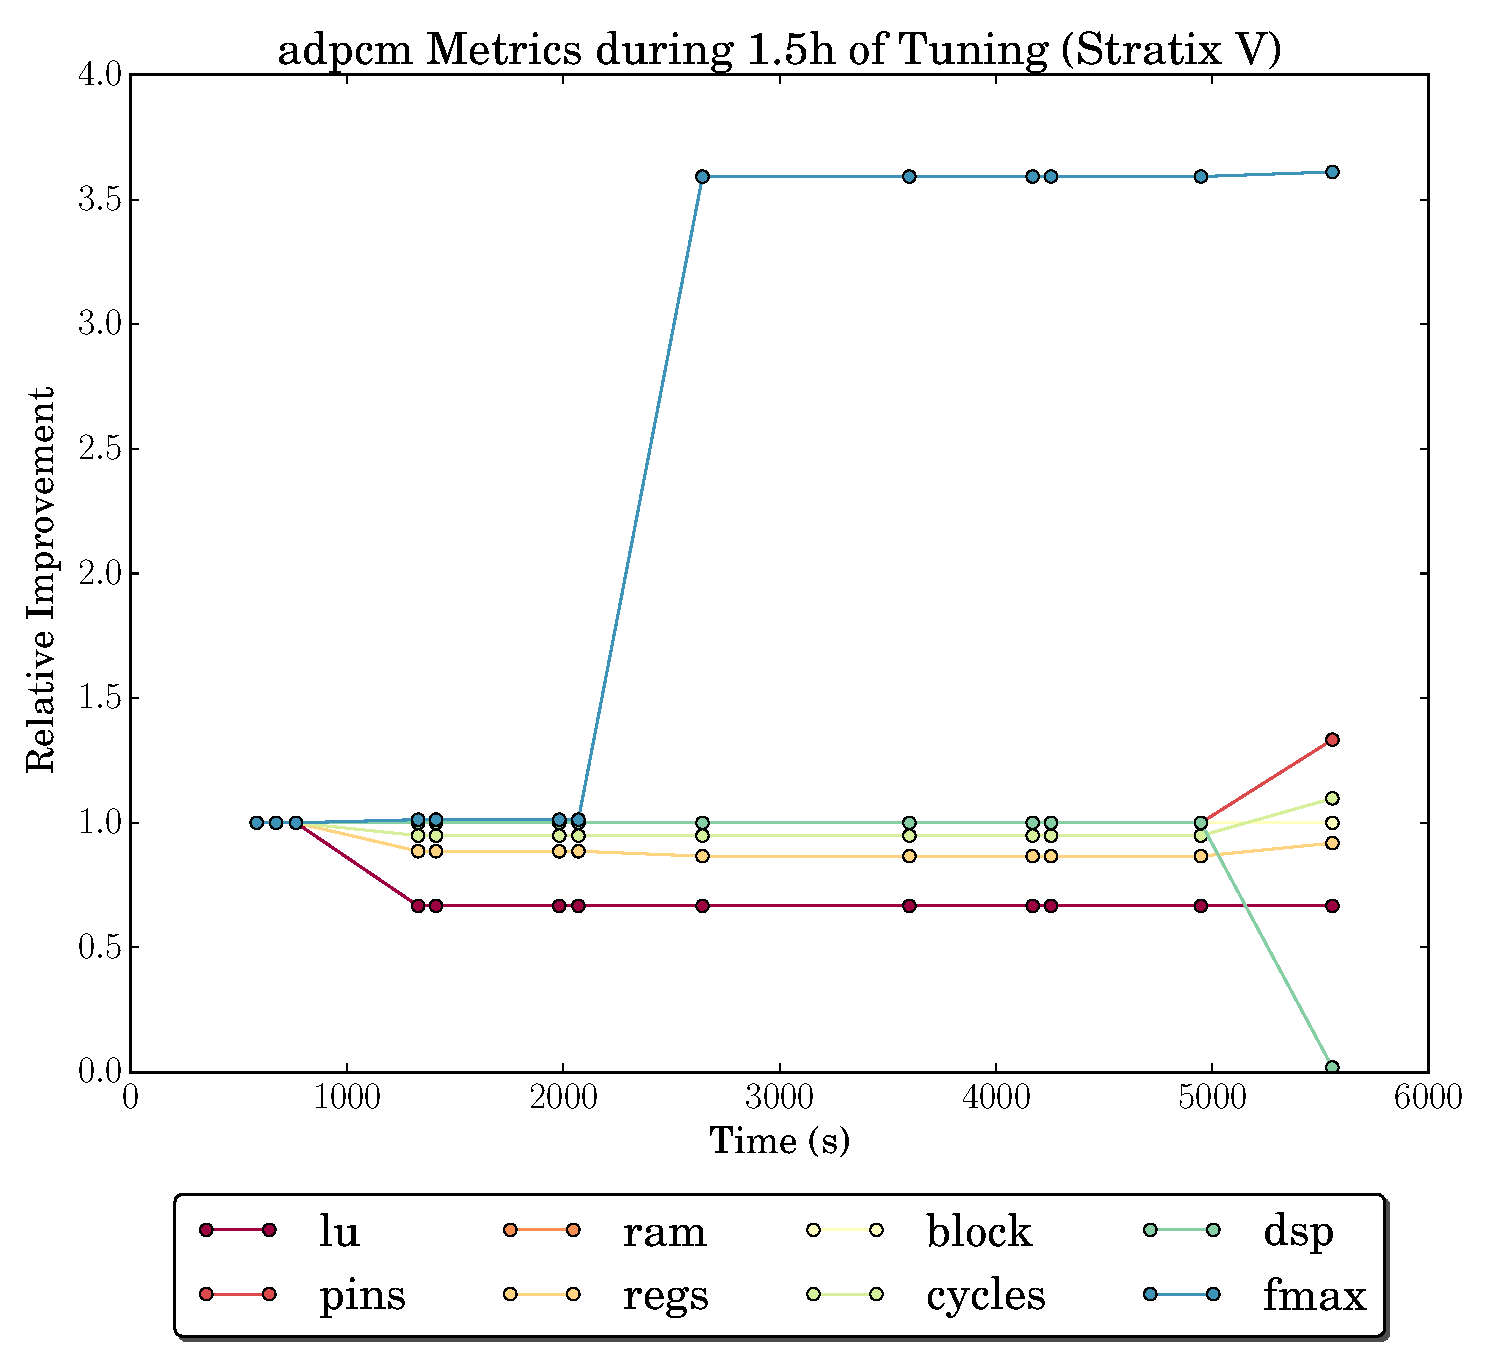
\includegraphics[width=.92\textwidth]{adpcm_all_5400_chstone_StratixV}
        \end{center}

        \column{0.5\textwidth}
        \begin{center}
            \includegraphics[width=.92\textwidth]{adpcm_all_5400_chstone_CycloneV}
        \end{center}

    \end{columns}
\end{frame}

\begin{frame}
    \frametitle{Results}
    Relative variation for the \alert{normalized sum of all metrics}
    of all CHStone application, after \alert{1.5h of tuning}:
    \begin{columns}[T,onlytextwidth]
        \column{0.5\textwidth}
        \begin{center}
            \includegraphics[width=.92\textwidth]{nsam_5400_chstone_StratixV}
        \end{center}

        \column{0.5\textwidth}
        \begin{center}
            \includegraphics[width=.92\textwidth]{nsam_5400_chstone_CycloneV}
        \end{center}

    \end{columns}
\end{frame}

\begin{frame}
    \frametitle{Results: Summary}
    Autotuning CHStone applications for the \alert{Stratix V DE5-Net} and
    \alert{Cyclone V DE1-SoC}:
    \begin{itemize}
        \item \alert{Different relative improvements} depending on \alert{board and application}
        \item From \alert{1\% up to 2x relative improvement} on the \alert{Normalized Sum of Metrics}
        \item Up to \alert{4x relative increase in frequency}
        \item Different relative improvements \alert{for each metric}
        \item Next: \alert{Select weights to target specific metrics}
    \end{itemize}
\end{frame}

\section{Next Steps: Expensive-to-Evaluate Functions}

\begin{frame}
    \frametitle{Next Steps: Expensive-to-Evaluate Functions}
    \begin{center}
        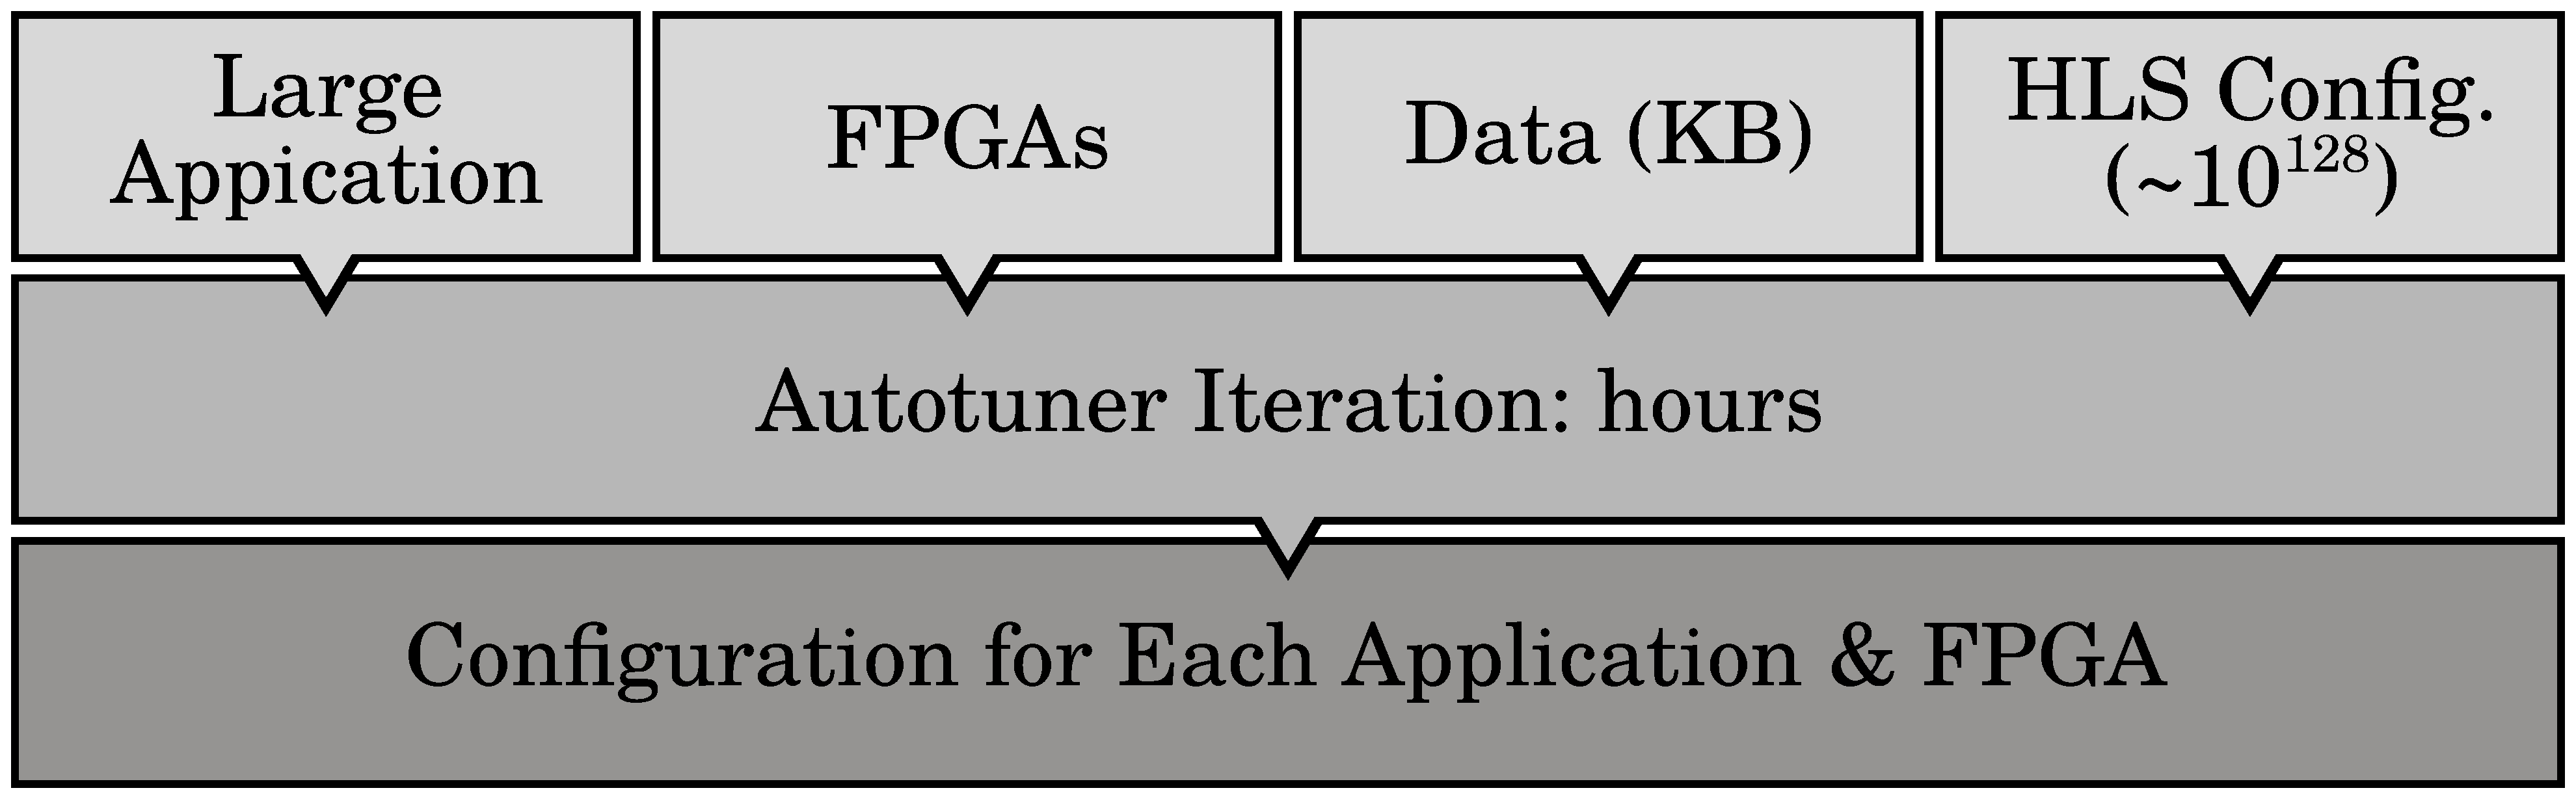
\includegraphics[width=.73\textwidth]{overview_fpgas_big}
    \end{center}

    \begin{itemize}
        \item \alert{1h} of tuning $\rightarrow \; \dfrac{1h}{\sim{}h} \approx \alert{1}$ \alert{iteration}
        \item Iterations now \alert{take too long}
    \end{itemize}
\end{frame}

\begin{frame}
    \frametitle{Next Steps: Expensive-to-Evaluate Functions}
    \alert{Design of Experiments}:
    \begin{itemize}
        \item With Arnaud Legrand and Jean-Marc Vincent
        \item Grenoble Université
        \item 2nd semester 2017
    \end{itemize}

    Future work:
    \begin{itemize}
        \item LLVM Passes for FPGAs
        \item Genetic Algorithm parameters
        \item Parallel and Distributed Autotuning
    \end{itemize}
\end{frame}

\begin{frame}
    \frametitle{Next Steps: Parallel and Distributed Autotuning}
    \begin{center}
        \includegraphics[width=.75\textwidth]{stochasticsearch_logo}
    \end{center}

    Domain-agnostic autotuning framework:
    \begin{itemize}
        \item \alert{Julia} language
        \item \alert{High Performance}, \alert{parallel and distributed computing}
        \item Using \alert{High-level abstractions}
        \item \alert{Expensive-to-evaluate} functions
        \item \url{github.com/phrb/StochasticSearch.jl}
    \end{itemize}
\end{frame}

\maketitle

\end{document}
